\iffalse
\documentclass[journal,12pt,twocolumn]{IEEEtran}
\usepackage{graphicx}
\graphicspath{{./chapters/10/7/4/1/figs/}}{}
\usepackage{amsmath,amssymb,amsfonts,amsthm}
\newcommand{\myvec}[1]{\ensuremath{\begin{pmatrix}#1\end{pmatrix}}}
\providecommand{\norm}[1]{\lVert#1\rVert}
\usepackage{listings}
\usepackage{watermark}
\usepackage{titlesec}
\usepackage{caption}
\let\vec\mathbf
\lstset{
frame=single, 
breaklines=true,
columns=fullflexible
}
\thiswatermark{\centering \put(0,-105.0){
\includegraphics[scale=0.15]{/sdcard/IITH/vector/vectpr-4/chapters/10/7/4/1/figs/logo.png}} }
\title{\mytitle}
\title{
Assignment - Vector-4
}
\author{Surajit Sarkar}
\begin{document}
\maketitle
%\tableofcontents
\bigskip
\section{\textbf{Problem}}
Determine the ratio in which the line 2x+y–4=0 divides the line segment joining the points A(2,–2) and B(3,7).
\section{\textbf{Solution}}
\begin{table}[h]
    \centering
    \begin{tabular}{|c|c|}
       \hline
       \textbf{Symbol}&\textbf{Value}  \\
       \hline
	    $\vec{A}$ & $\myvec{2\\-2}$\\
        \hline
	    $\vec{B}$ & $\myvec{3\\7}$\\
        \hline
	    c&$4$\\
        \hline
       $\vec{n}$ & $\myvec{2\\1}$\\
       \hline
    \end{tabular}
    \caption{Parameters}
    \label{tab:my_label}
\end{table}
Given equation
\fi
The given equation can be expressed as
\begin{align}
    \myvec{2&1}\vec{x}&=4\\
\end{align}
Using section formula, the point of division 
\begin{align}
    \vec{P} = \frac{k\vec{B+A}}{k+1}
\end{align}
which upon substitution in the equation of a line yields
\begin{align}
    \implies\vec{n}^{\top}\myvec{\frac{k\vec{B+A}}{k+1}}&=c\\
    \implies k&=\frac{c-\vec{n}^{\top}\vec{A}}{\vec{n}^{\top}\vec{B}-c}\\
\end{align}
upon simplification.  Substituting numerical values, 
\begin{align}
    k=\frac{2}{9}
\end{align}
See Fig. 
\ref{fig:chapters/10/7/4/1vec}.
\begin{figure}[!h]
\centering
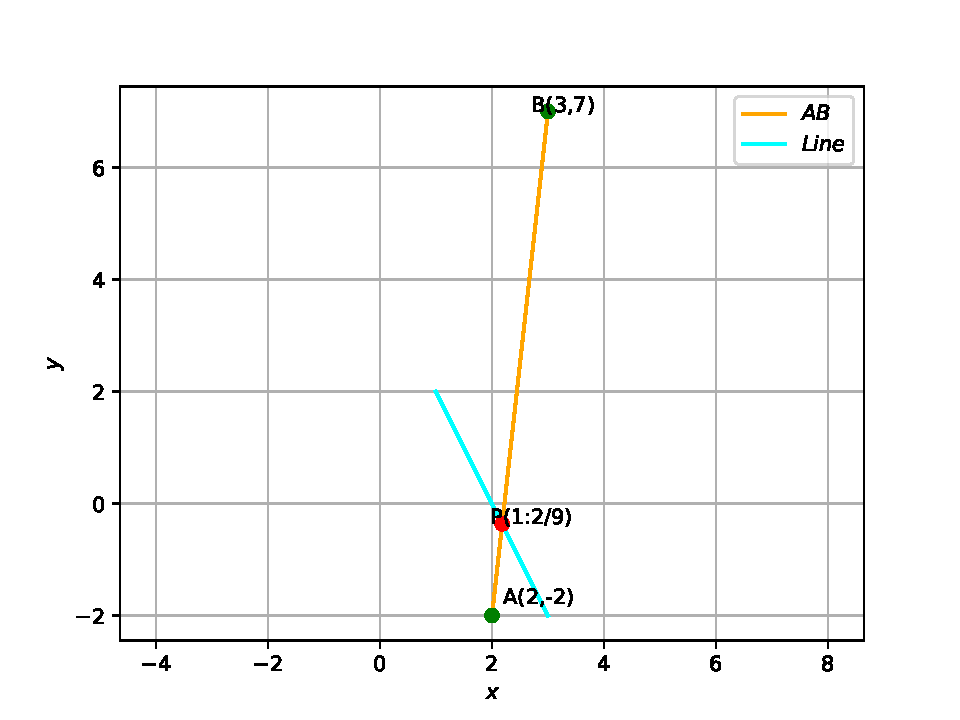
\includegraphics[width=\columnwidth]{chapters/10/7/4/1/figs/vec.pdf}
\caption{}
\label{fig:chapters/10/7/4/1vec}
\end{figure}

